\chapter*{Shanghai\markboth{Shanghai}{}}
\section*{14 septembre 2015}
Beaucoup de sites internet comme Google, Twitter ou Facebook sont bloqués en Chine, heureusement le blog est accessible !

 Après un court vol de 3h j'atteris à Shanghai. Première impression, des infrastructures très modernes partout, des immeubles très hauts, pas une ambiance vraiment chinoise 

 

\begin{center} 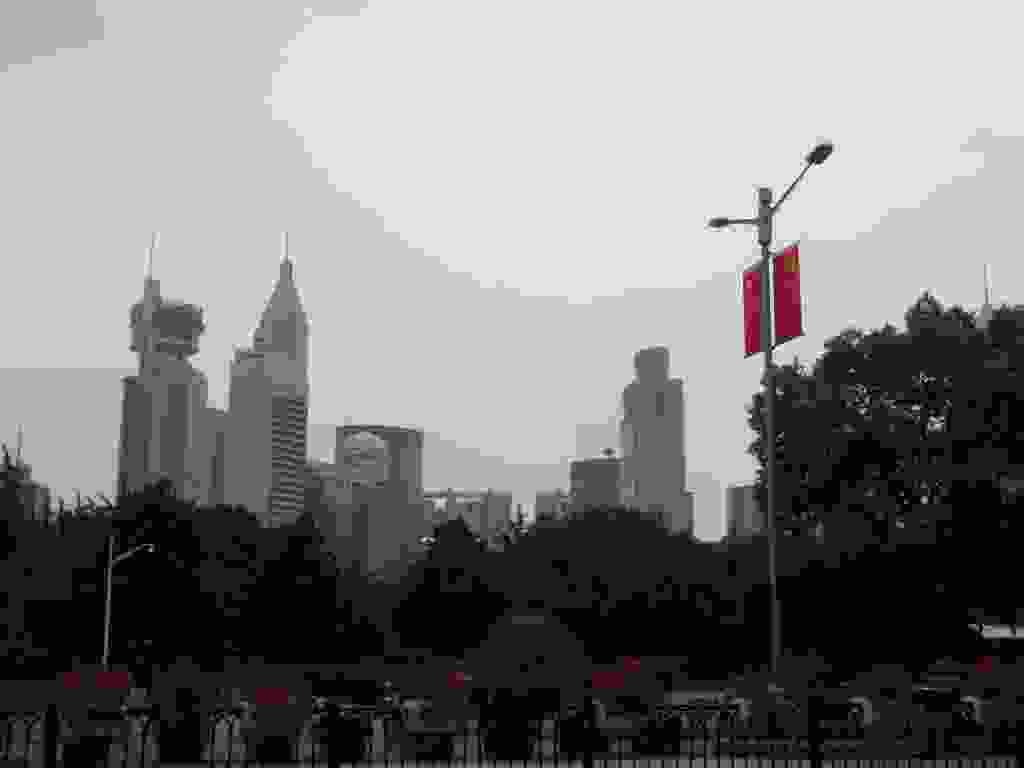
\includegraphics[width=\mywidth]{../wp-content/uploads/2015/09/P8316550-1024x768.jpg} \end{center}

 

 Pas de vélo ici, le métro est pratique et sécurisé, il y a même une vérification des sacs à l'entrée 

 

\begin{center} 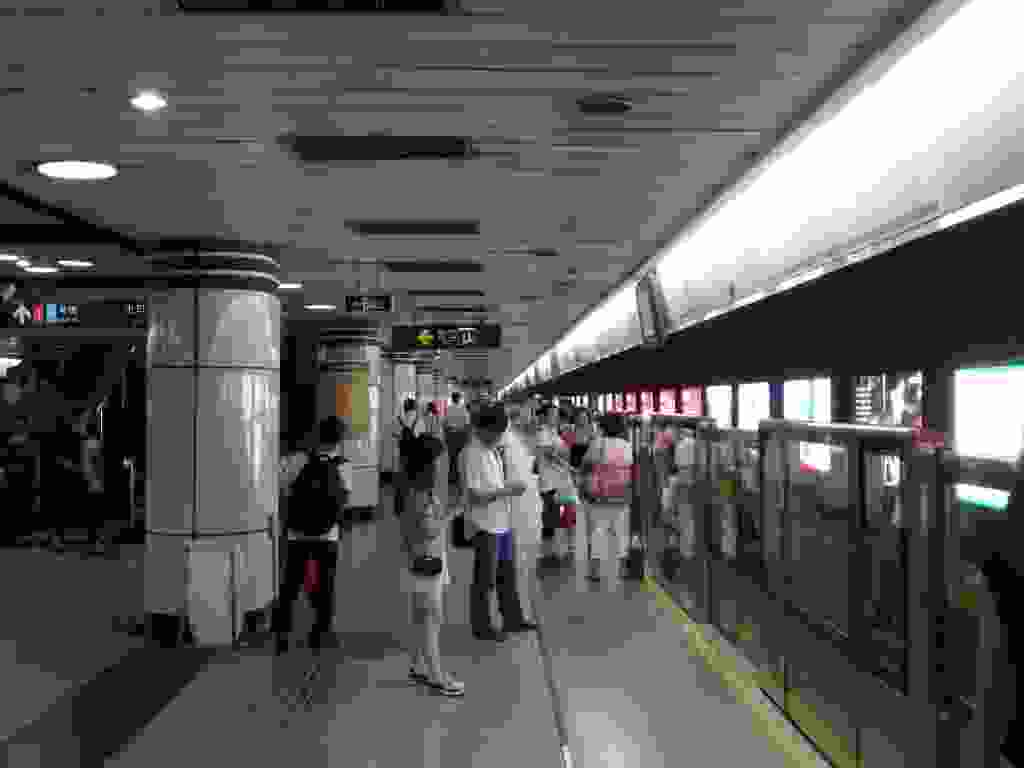
\includegraphics[width=\mywidth]{../wp-content/uploads/2015/09/P9016606-1024x768.jpg} \end{center}

 

 Je suis hébergé dans le quartier de la concession francaise, agréable avec beaucoup d'arbres 

 

\begin{center} 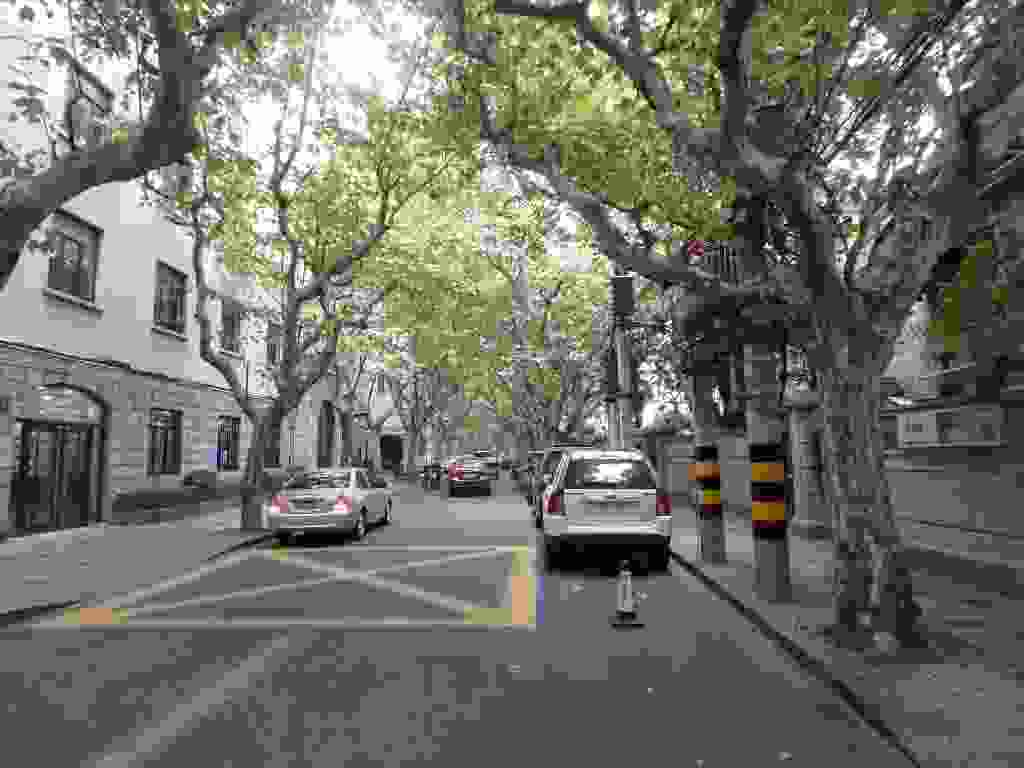
\includegraphics[width=\mywidth]{../wp-content/uploads/2015/09/P8316529-1024x768.jpg} \end{center}

 

 Je commence par une balade dans le parc Fu Xing le matin. 

 

\begin{center} 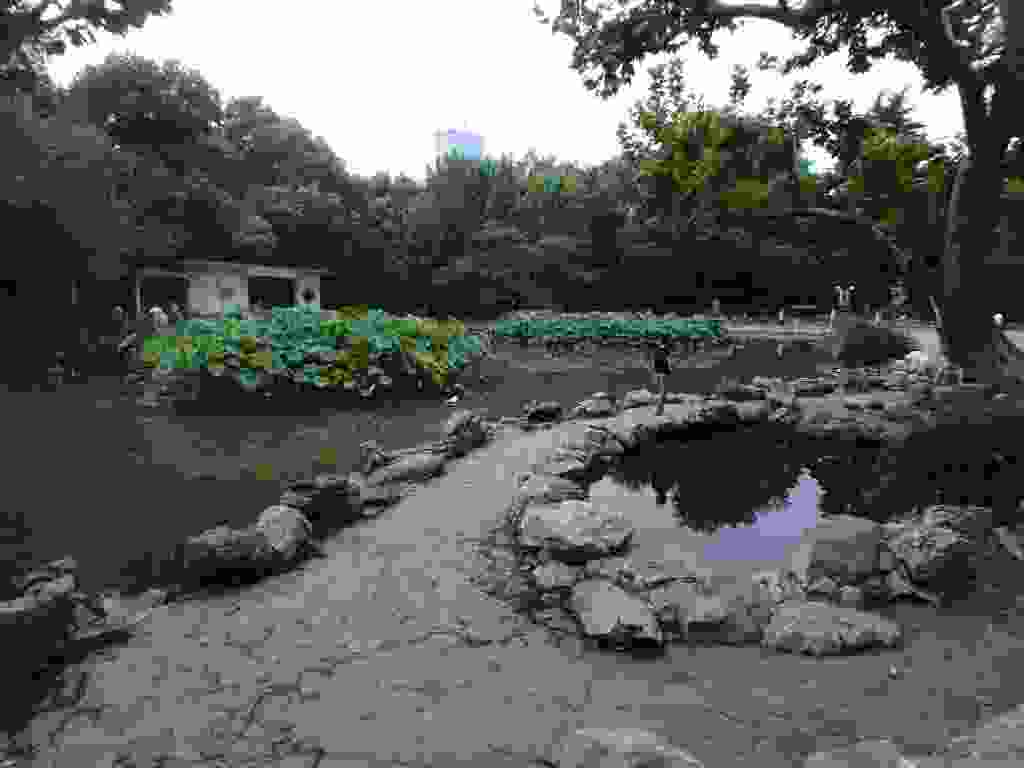
\includegraphics[width=\mywidth]{../wp-content/uploads/2015/09/P8316533-1024x768.jpg} \end{center}

 

 Les gens s'adonnent à tous types d'activités 

 

\begin{center} 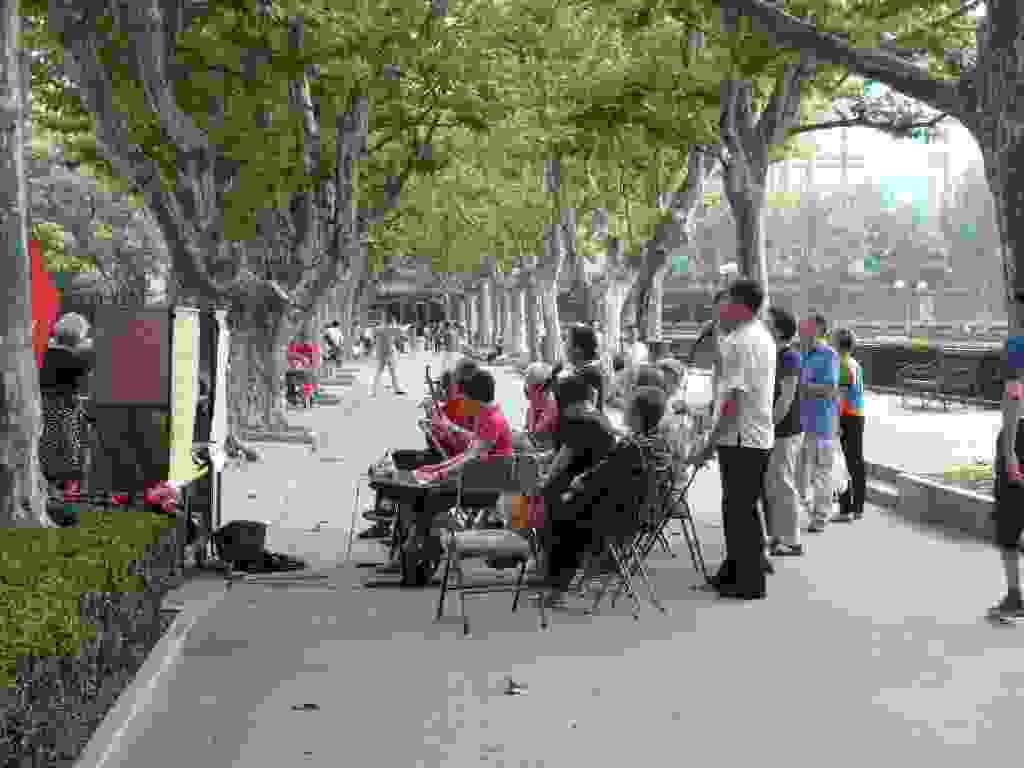
\includegraphics[width=\mywidth]{../wp-content/uploads/2015/09/P8316536-1024x768.jpg} \end{center}

 

 

\begin{center} 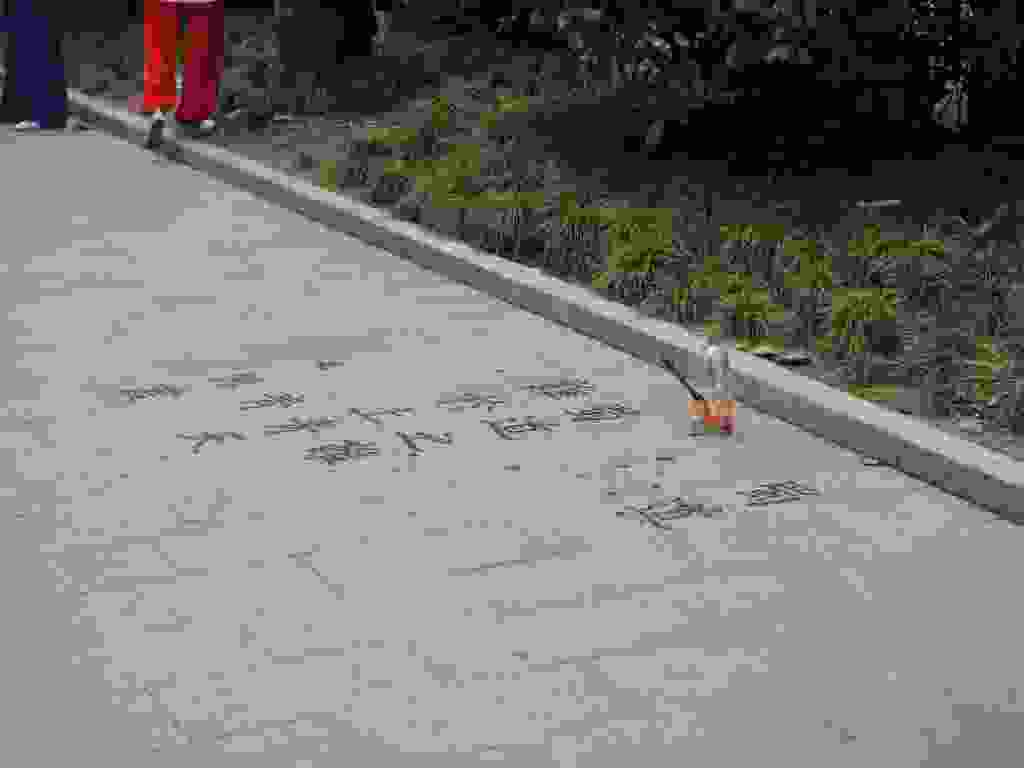
\includegraphics[width=\mywidth]{../wp-content/uploads/2015/09/P8316538-1024x768.jpg} \end{center}

 

 

\begin{center} 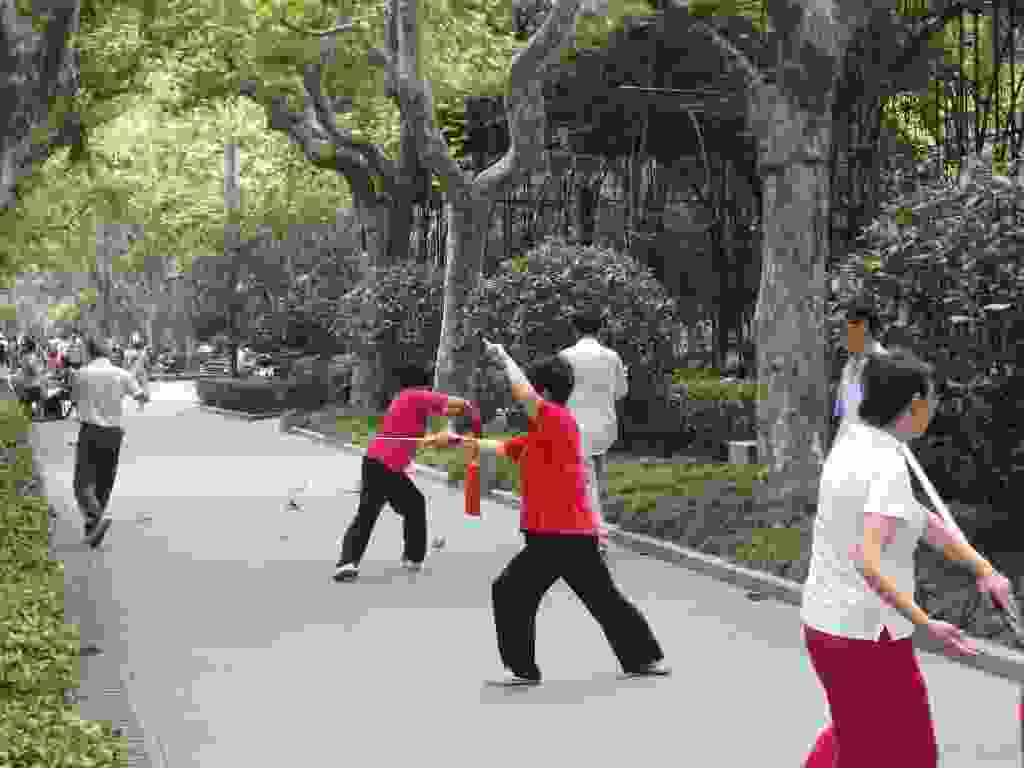
\includegraphics[width=\mywidth]{../wp-content/uploads/2015/09/P8316539-1024x768.jpg} \end{center}

 

 

\begin{center} 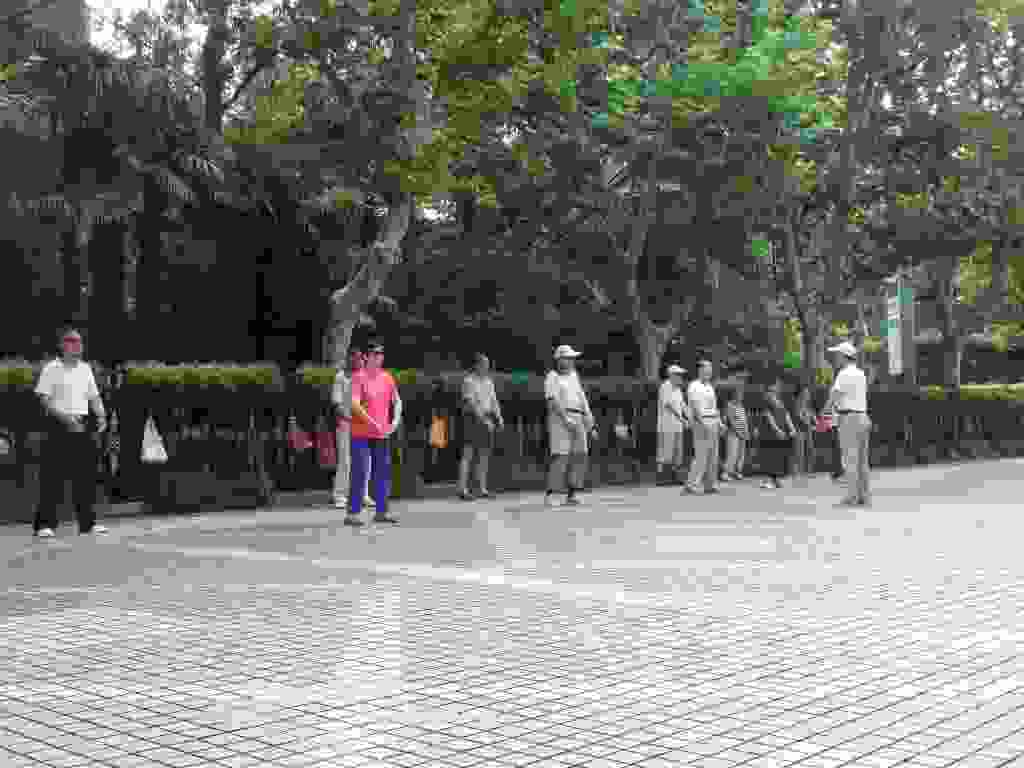
\includegraphics[width=\mywidth]{../wp-content/uploads/2015/09/P8316541-1024x768.jpg} \end{center}

 

 

\begin{center} 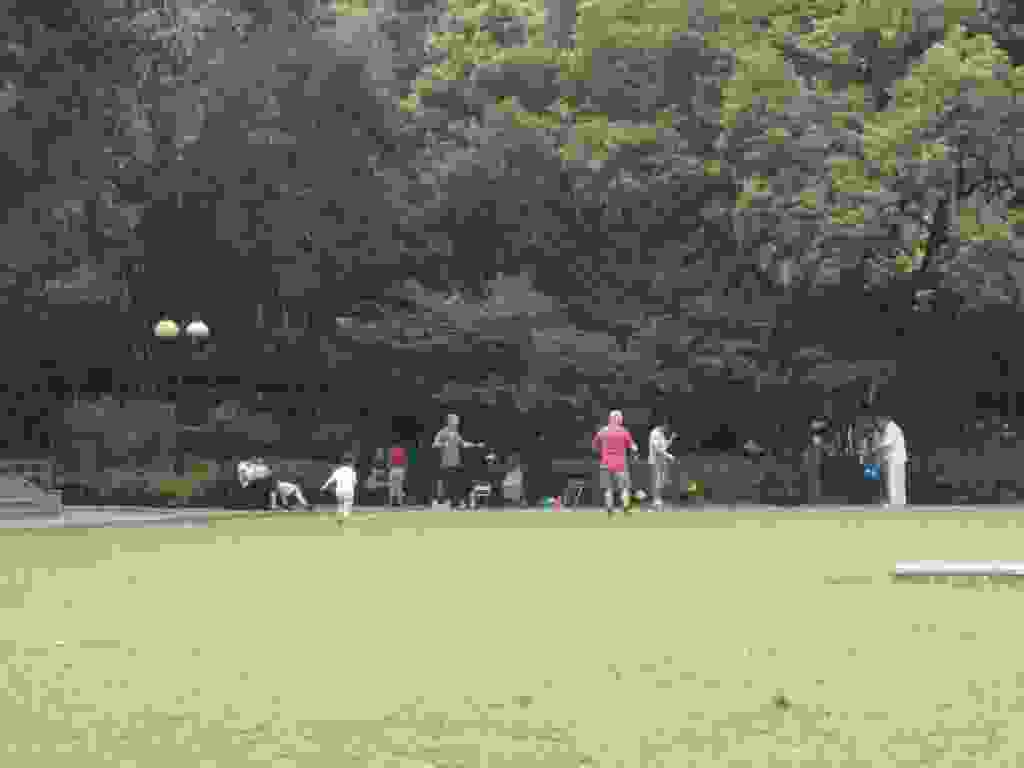
\includegraphics[width=\mywidth]{../wp-content/uploads/2015/09/P8316542-1024x768.jpg} \end{center}

 

 People's Square, la place principale de Shanghai 

 

\begin{center} 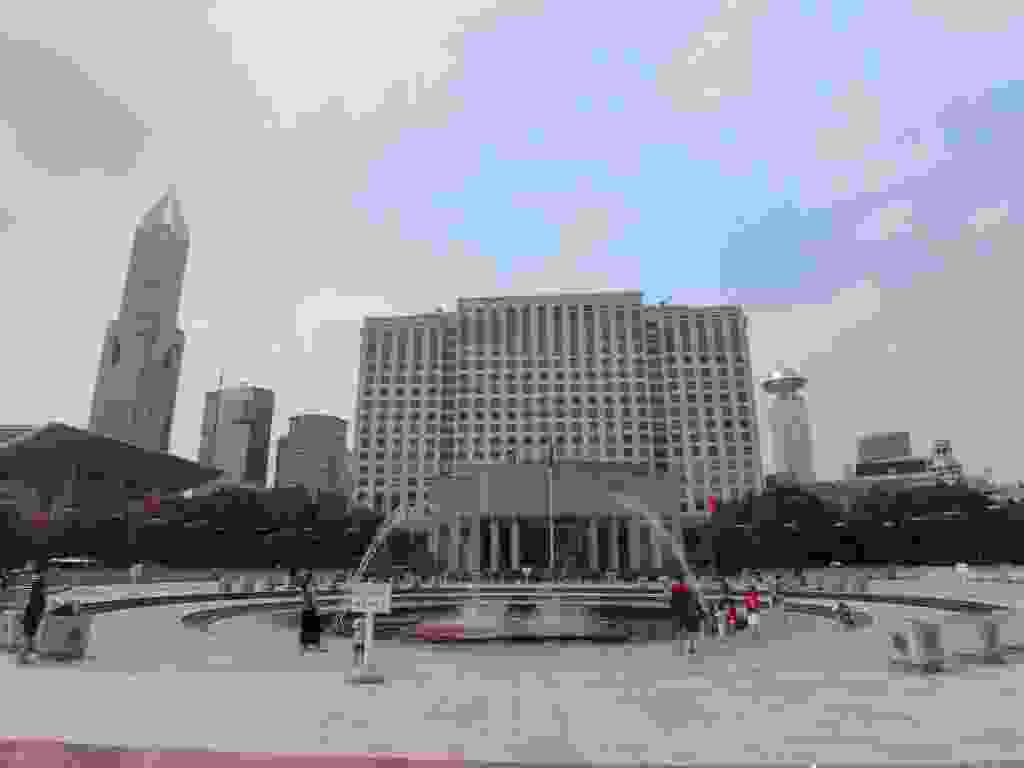
\includegraphics[width=\mywidth]{../wp-content/uploads/2015/09/P8316552-1024x768.jpg} \end{center}

 

 C'est là que se trouve le Shanghai Museum 

 

\begin{center} 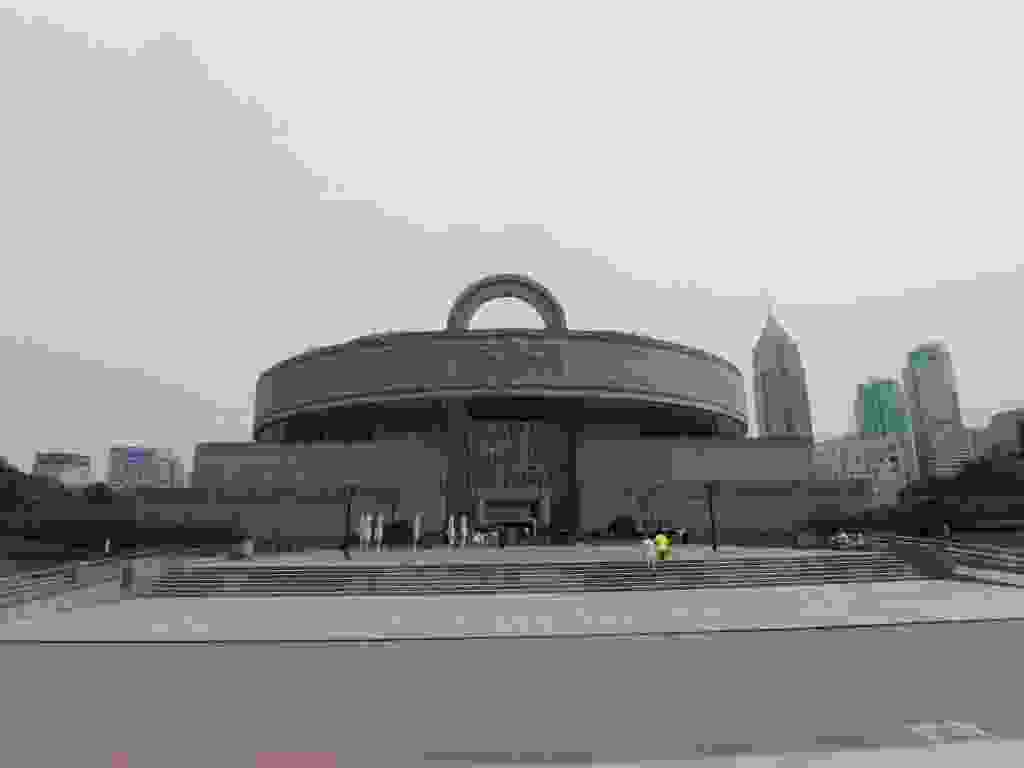
\includegraphics[width=\mywidth]{../wp-content/uploads/2015/09/P8316553-1024x768.jpg} \end{center}

 

 

\begin{center} 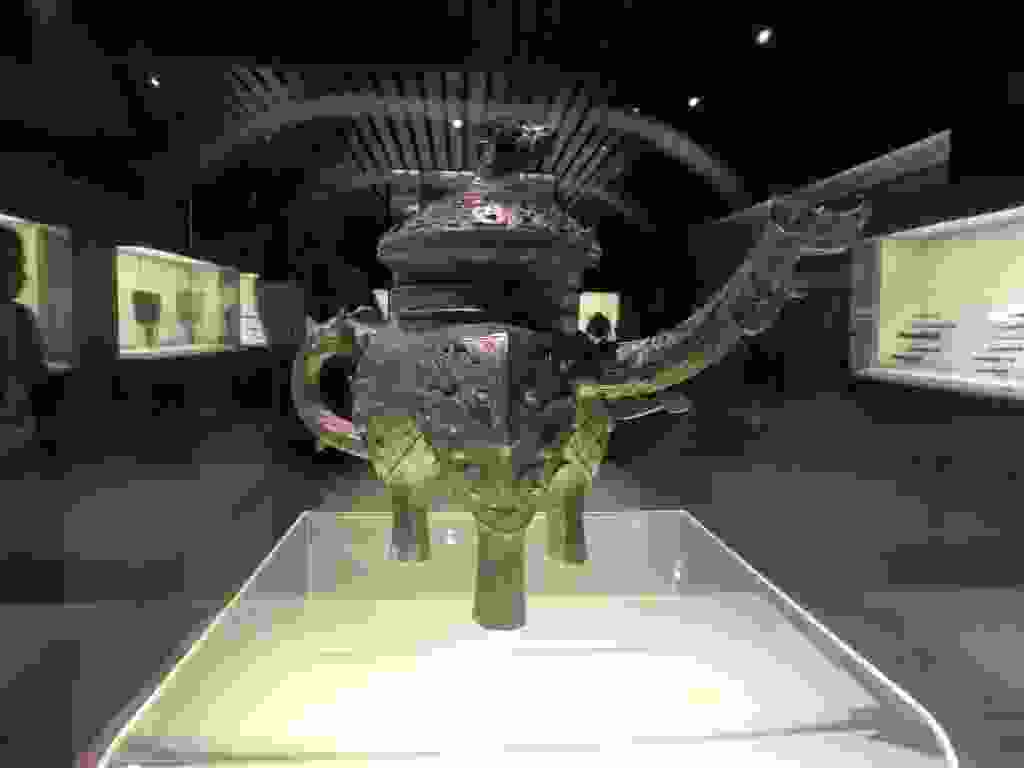
\includegraphics[width=\mywidth]{../wp-content/uploads/2015/09/P8316556-1024x768.jpg} \end{center}

 

 

\begin{center} 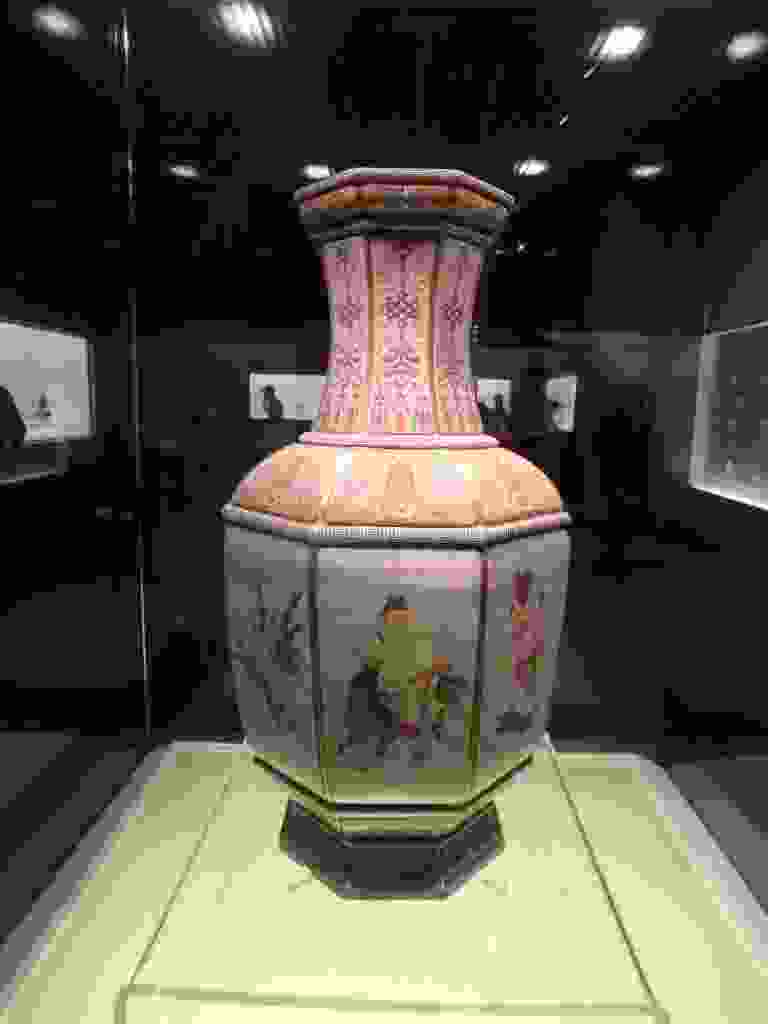
\includegraphics[width=\mywidth]{../wp-content/uploads/2015/09/P8316558-e1441267394556-768x1024.jpg} \end{center}

 

 

\begin{center} 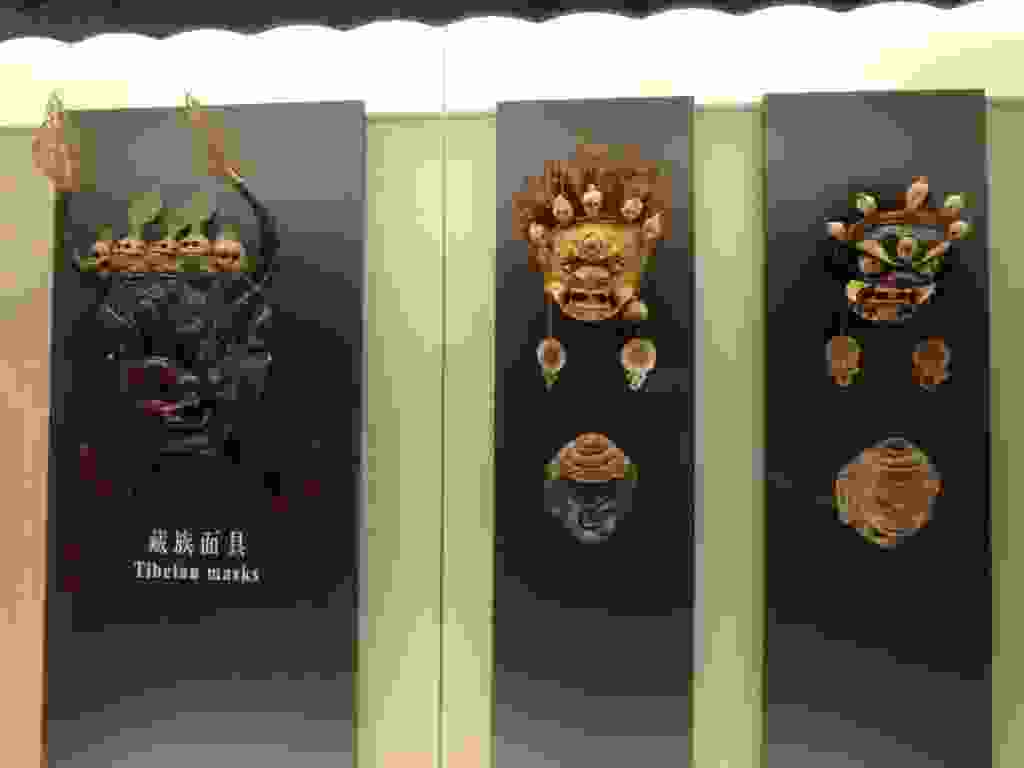
\includegraphics[width=\mywidth]{../wp-content/uploads/2015/09/P8316560-1024x768.jpg} \end{center}

 

 

\begin{center} 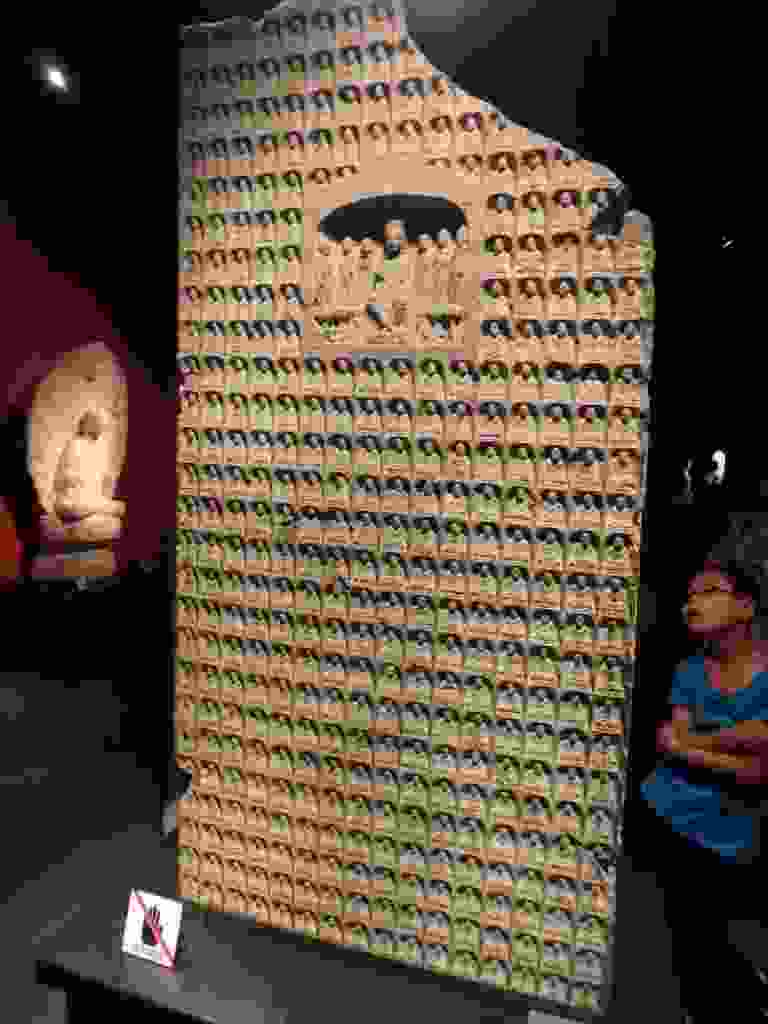
\includegraphics[width=\mywidth]{../wp-content/uploads/2015/09/P8316561-e1441455299605-768x1024.jpg} \end{center}

 

 La Nanjing Road, rue touristique avec des boutiques 

 C'est dans cette rue que j'observe 2 fois la tentative d'arnaque classique de Shanghai : un groupe de jeunes chinois très sympatiques et parlant bien anglais viennent discuter, après un bon moment ils me proposent de venir boire un thé. Comme j'étais prévenu je ne les ai pas suivi mais le principe est ensuite de faire payer une addition exhorbitante pour le thé. 

 

\begin{center} 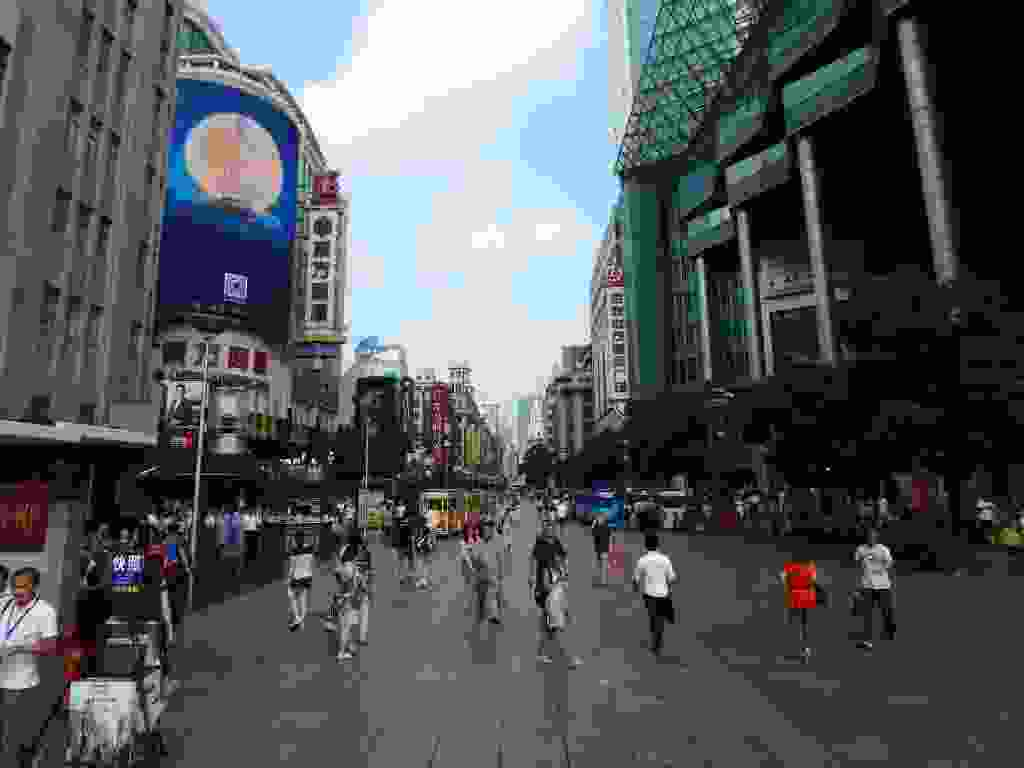
\includegraphics[width=\mywidth]{../wp-content/uploads/2015/09/P8316564-1024x768.jpg} \end{center}

 

 La rue se termine sur The Bund avec la vue la plus célèbre de Shanghai 

 

\begin{center} 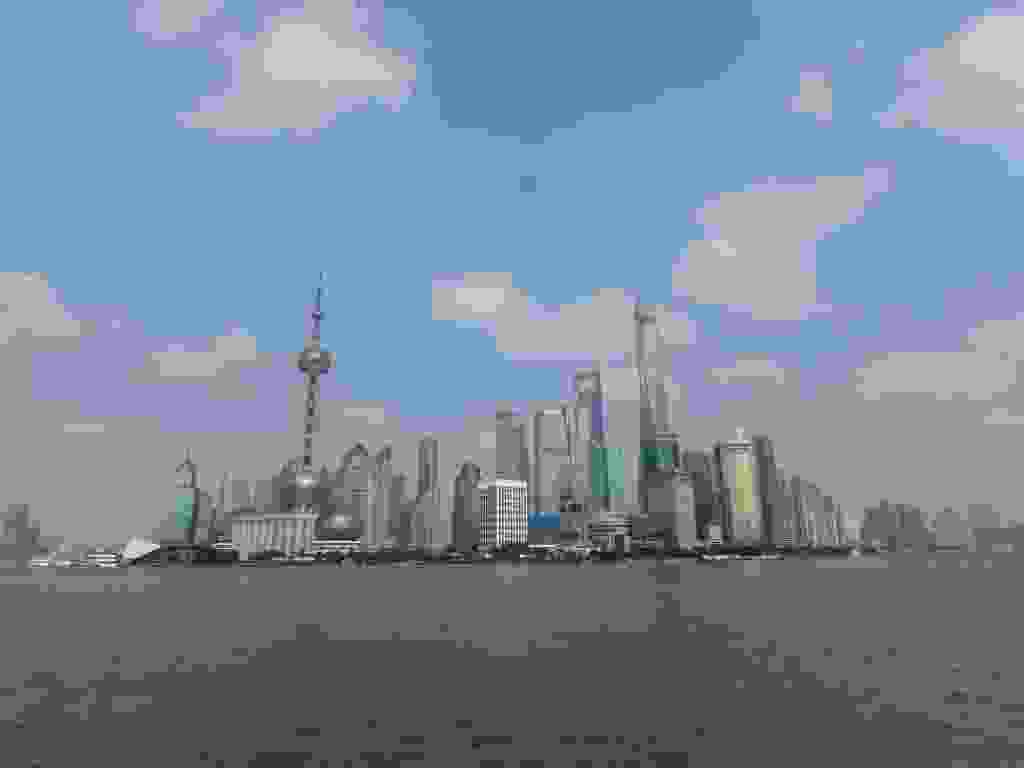
\includegraphics[width=\mywidth]{../wp-content/uploads/2015/09/P8316565-1024x768.jpg} \end{center}

 

 

\begin{center} 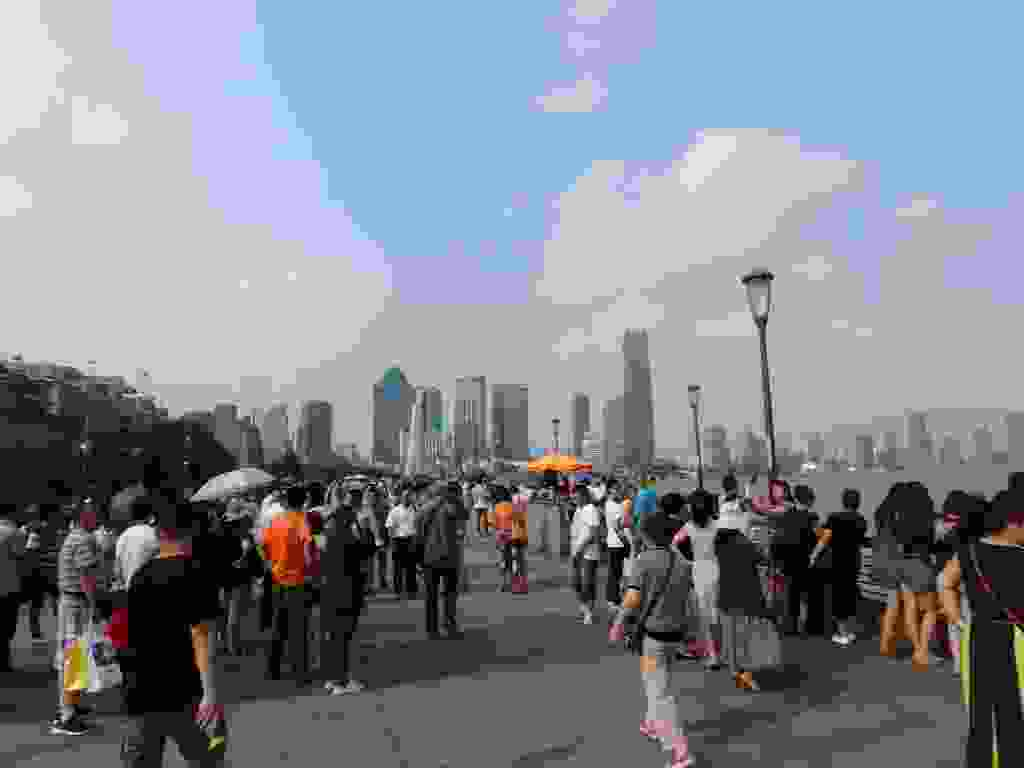
\includegraphics[width=\mywidth]{../wp-content/uploads/2015/09/P8316568-1024x768.jpg} \end{center}

 

 Yuyuan : le quartier traditionnel chinois 

 

\begin{center} 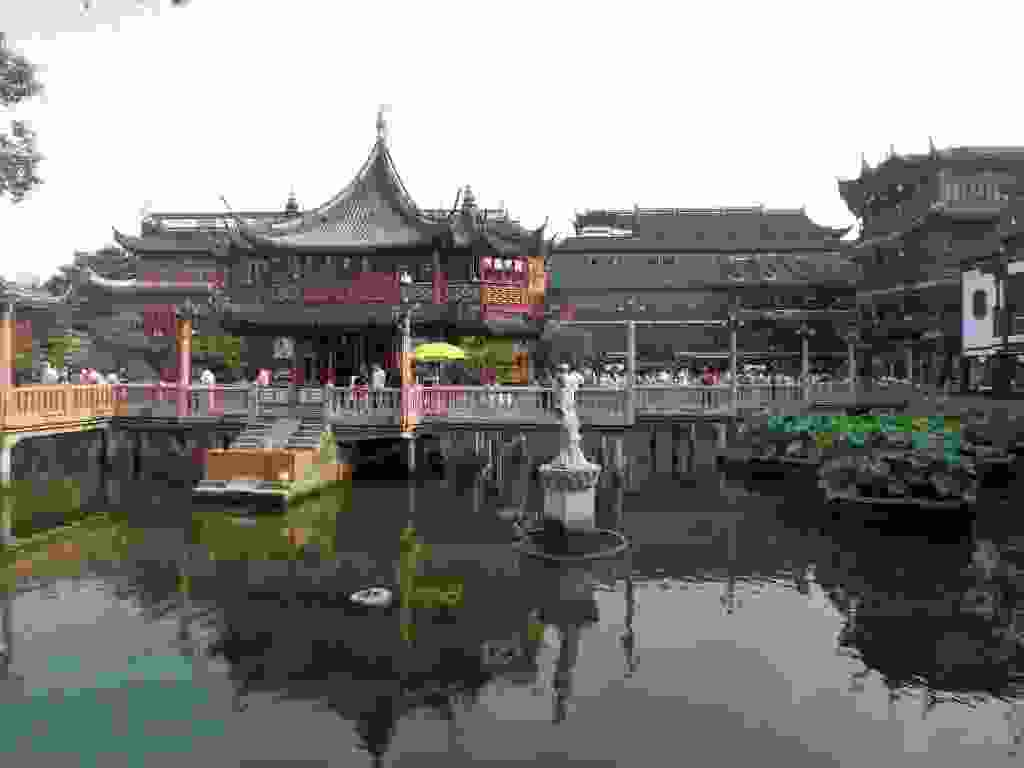
\includegraphics[width=\mywidth]{../wp-content/uploads/2015/09/P8316576-1024x768.jpg} \end{center}

 

 

\begin{center} 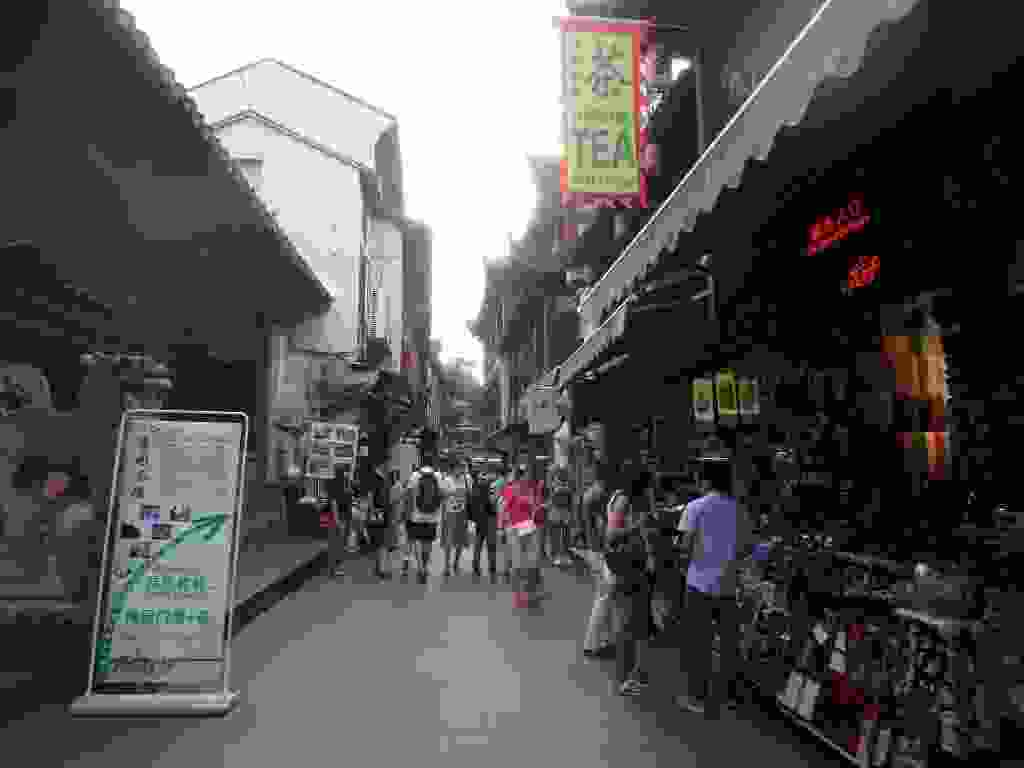
\includegraphics[width=\mywidth]{../wp-content/uploads/2015/09/P8316594-1024x768.jpg} \end{center}

 

 

\begin{center} 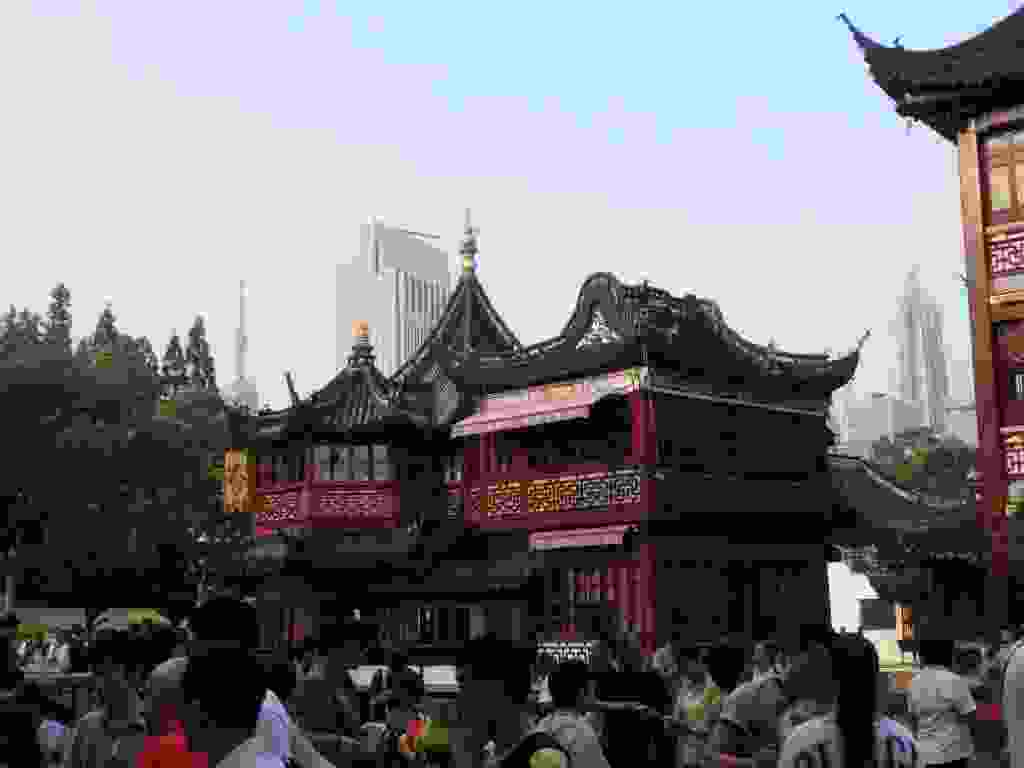
\includegraphics[width=\mywidth]{../wp-content/uploads/2015/09/P8316596-1024x768.jpg} \end{center}

 

 

\begin{center} 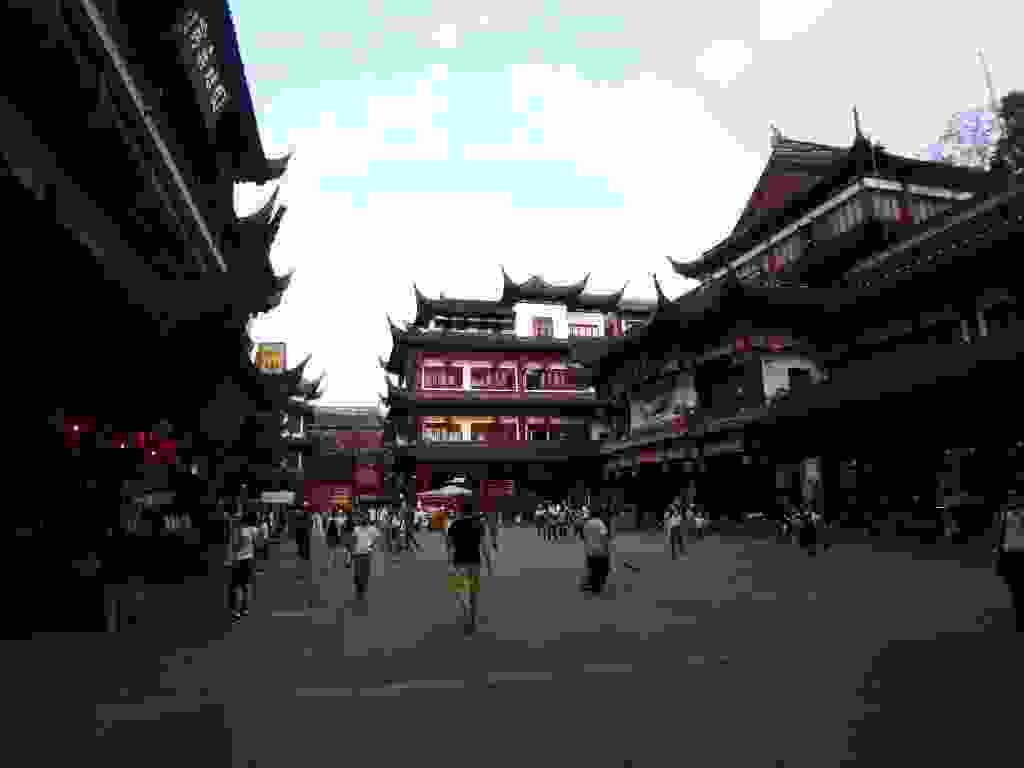
\includegraphics[width=\mywidth]{../wp-content/uploads/2015/09/P8316598-1024x768.jpg} \end{center}

 

 Le jardin Yu avec ses petits pavillons typiques 

 

\begin{center} 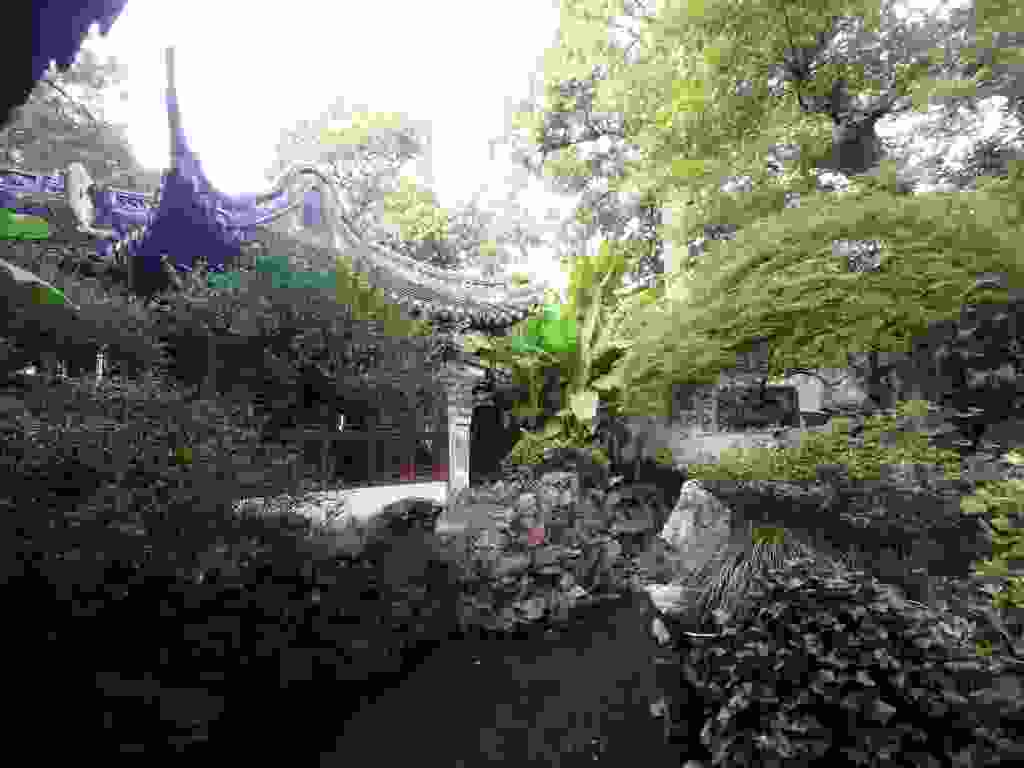
\includegraphics[width=\mywidth]{../wp-content/uploads/2015/09/P8316579-1024x768.jpg} \end{center}

 

 

\begin{center} 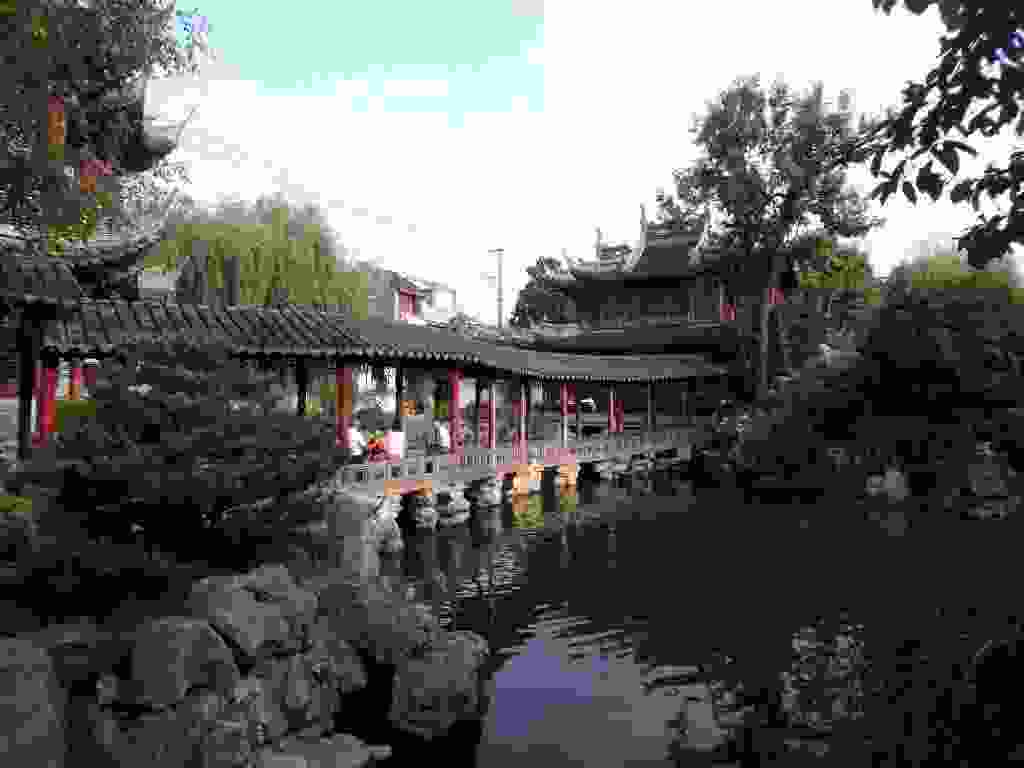
\includegraphics[width=\mywidth]{../wp-content/uploads/2015/09/P8316585-1024x768.jpg} \end{center}

 

 

\begin{center} 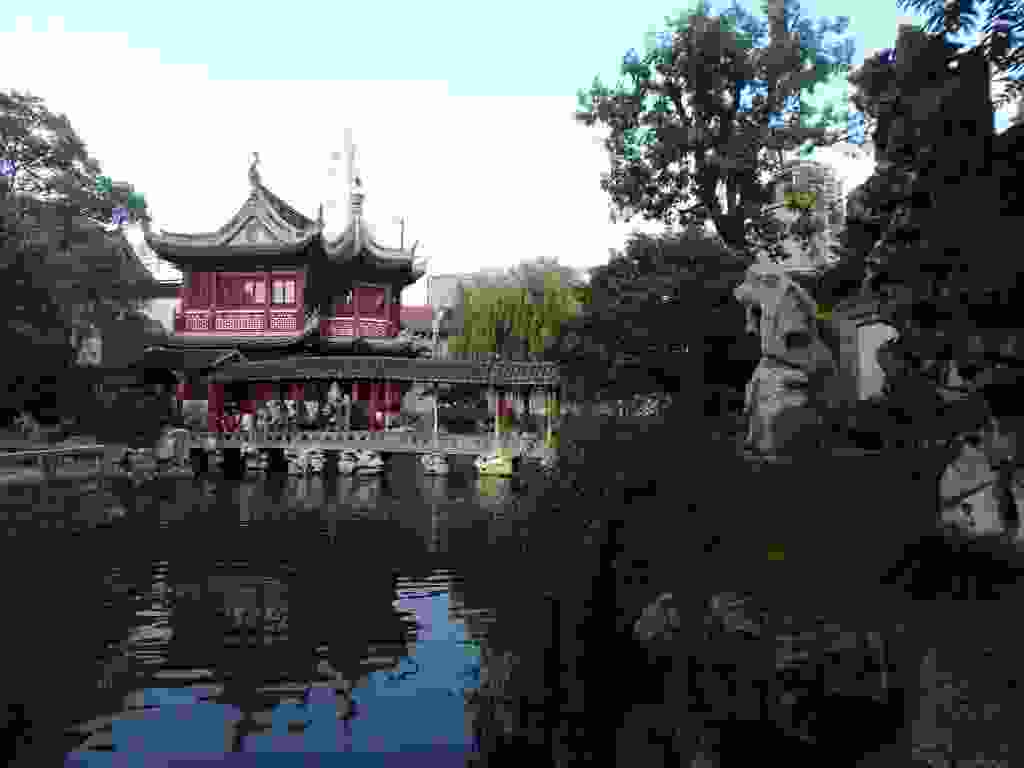
\includegraphics[width=\mywidth]{../wp-content/uploads/2015/09/P8316588-1024x768.jpg} \end{center}

 

 Des animaux sympatiques au marché 

 

\begin{center} 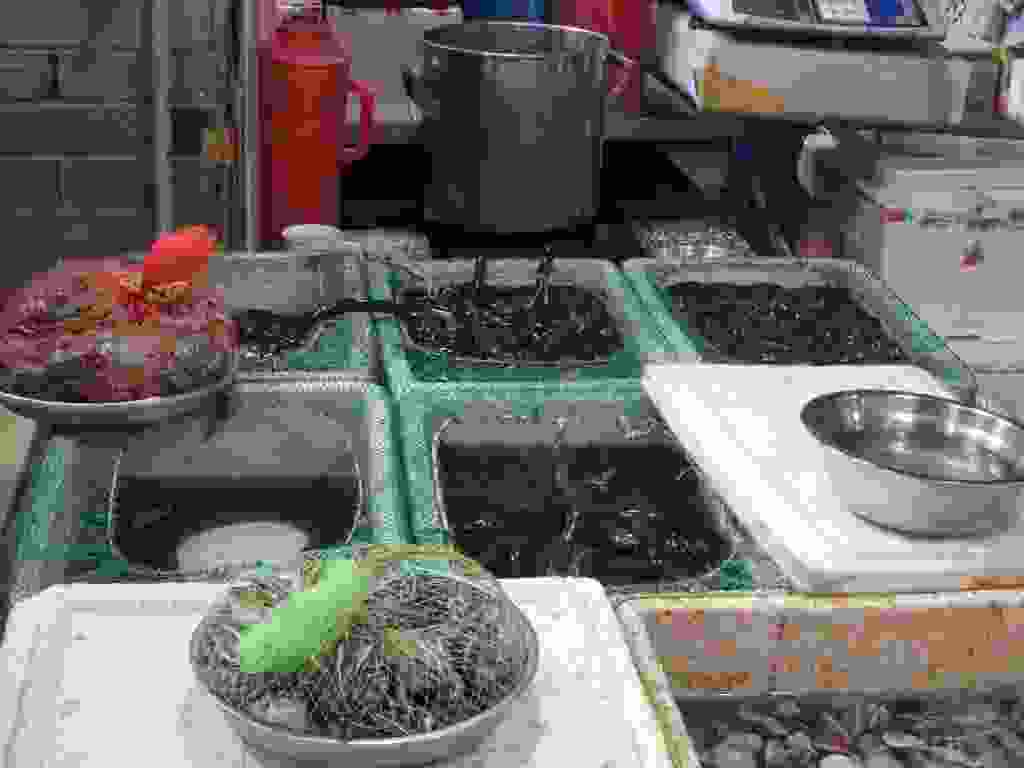
\includegraphics[width=\mywidth]{../wp-content/uploads/2015/09/P9016603-1024x768.jpg} \end{center}

 

 J'ai été accueilli en Warmshowers par Kyle, américain qui organise des visites gastronomiques de Shanghai. Il m'a invité à venir avec sa collègue à une soirée repérage de restaurants, de belles découvertes ! 

 

\begin{center} 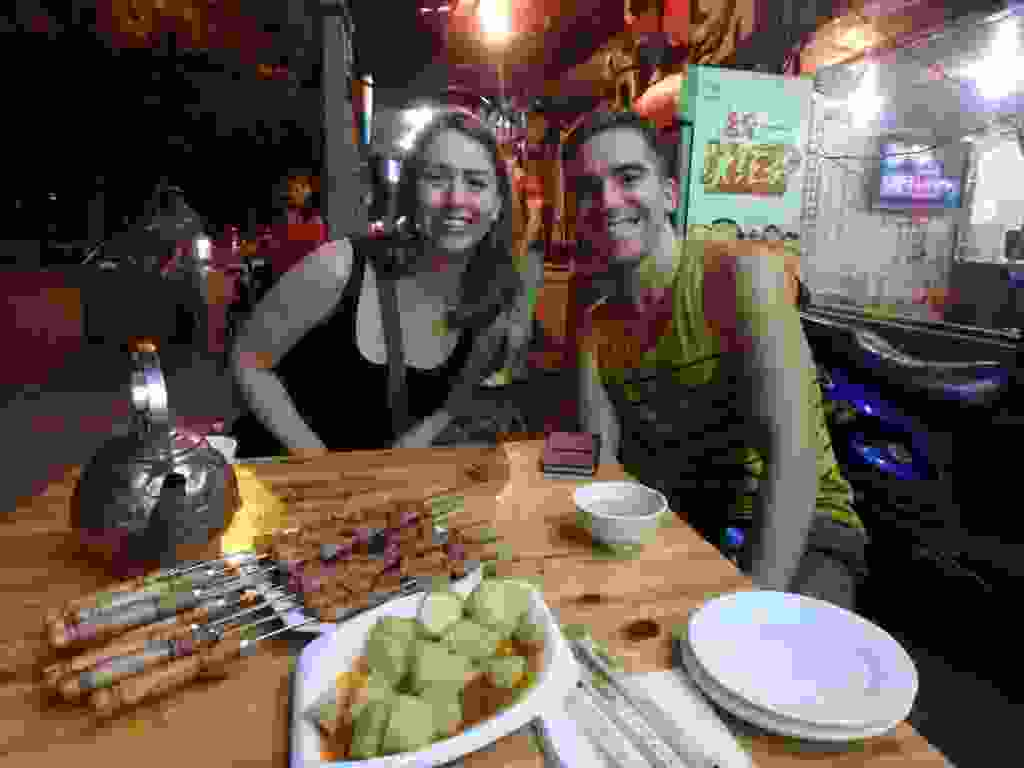
\includegraphics[width=\mywidth]{../wp-content/uploads/2015/09/P9016614-1024x768.jpg} \end{center}

 

 Le ping pong est le sport national en Chine, il faut bien que j'essaye d'aller taper la balle : 

 D'abord acheter une raquette chinoise pas chère 

 

\begin{center} 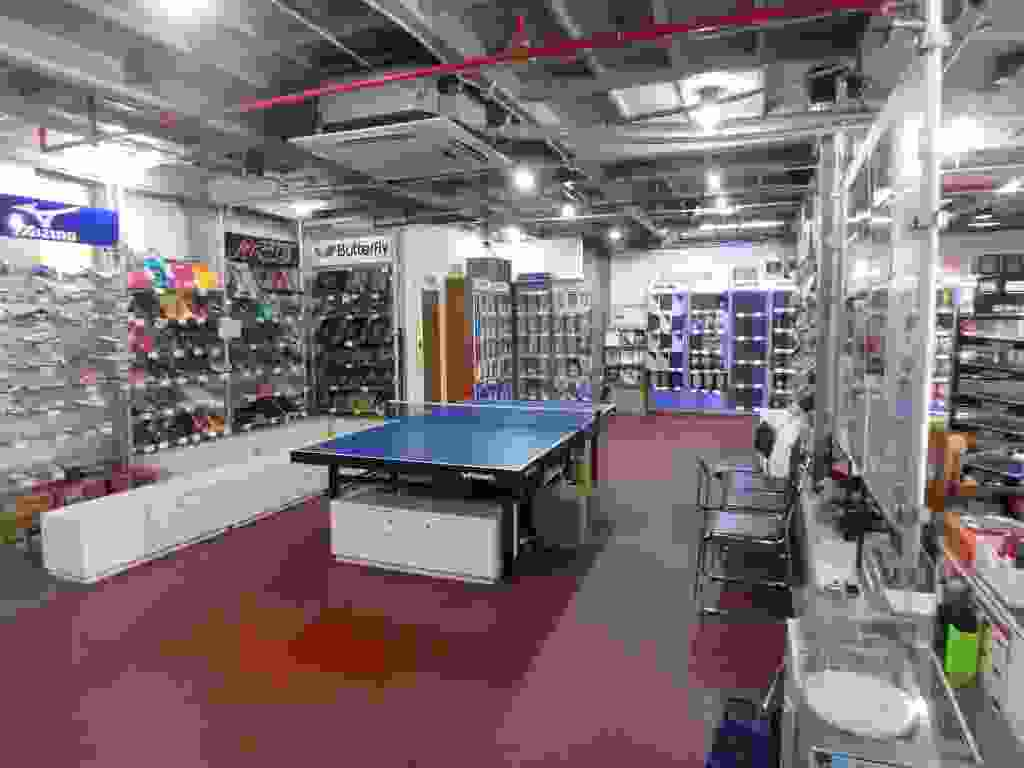
\includegraphics[width=\mywidth]{../wp-content/uploads/2015/09/P9016604-1024x768.jpg} \end{center}

 

 Puis trouver une salle pour jouer un peu, il n'y avait pas trop de monde, bon niveau mais sans plus 

 

\begin{center} 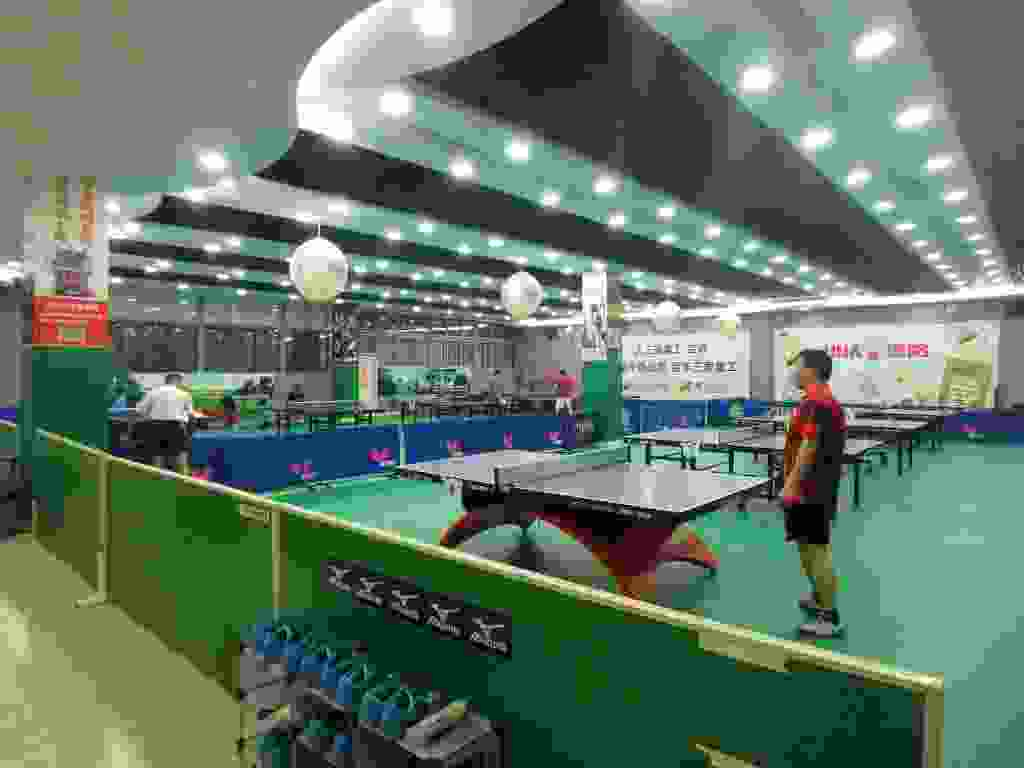
\includegraphics[width=\mywidth]{../wp-content/uploads/2015/09/P9016609-1024x768.jpg} \end{center}

 

 Je quitte Shanghai pour 21h de train direction Xi'an 

 

\begin{center} 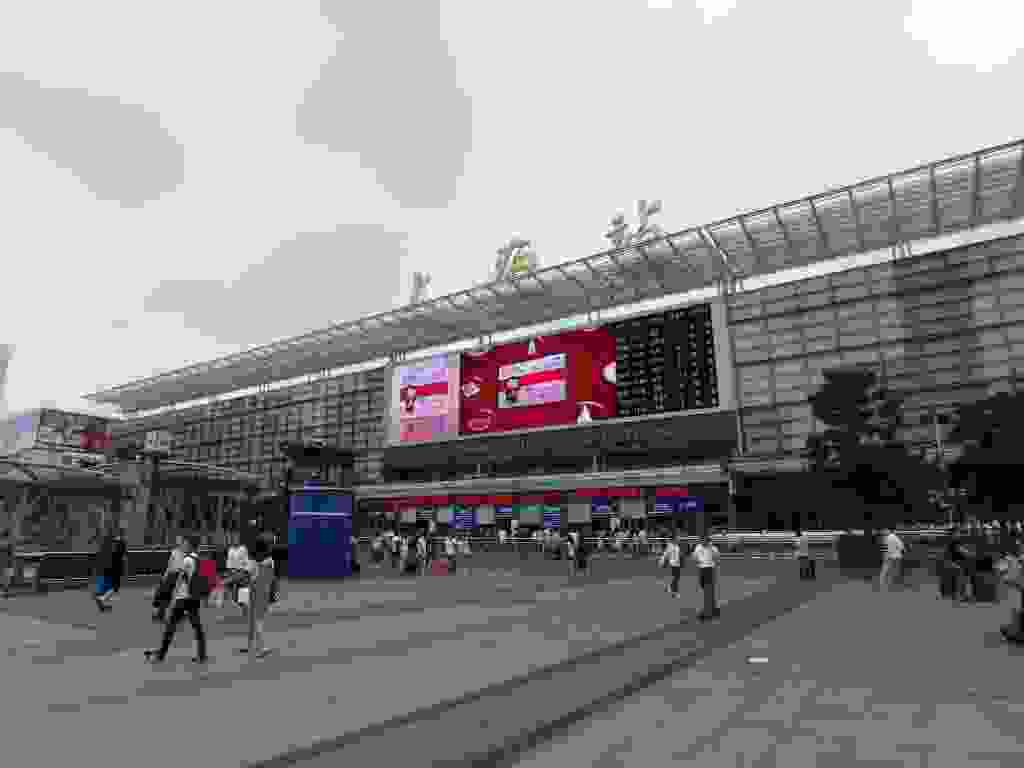
\includegraphics[width=\mywidth]{../wp-content/uploads/2015/09/P8316548-1024x768.jpg} \end{center}

 

 

\begin{center} 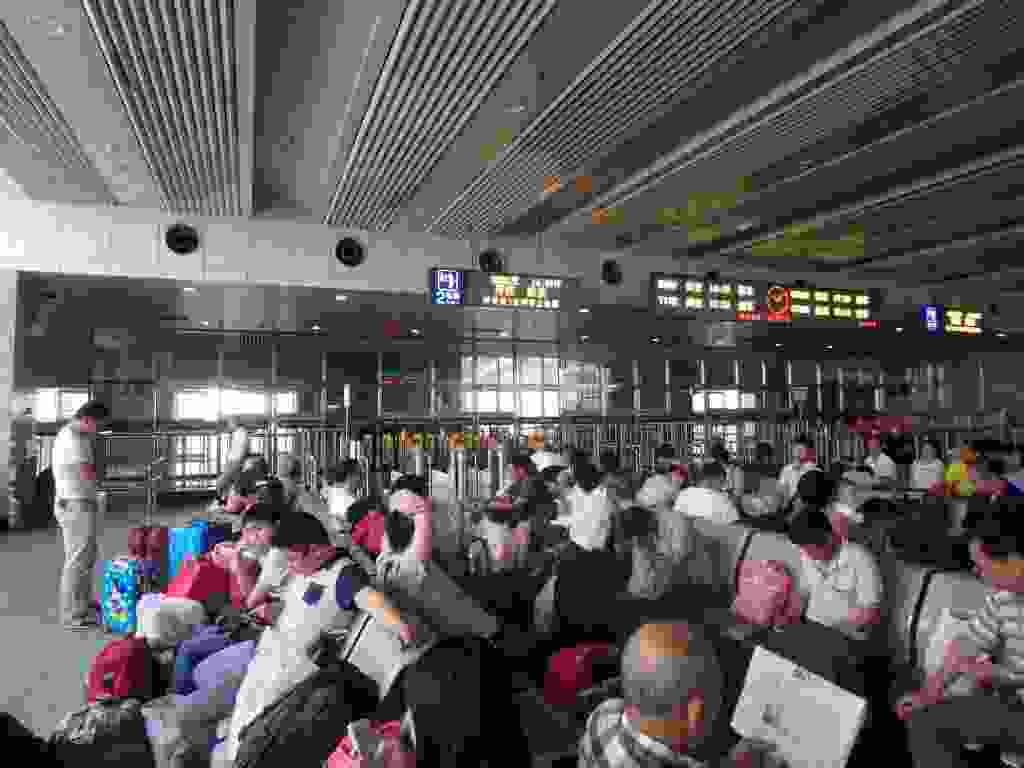
\includegraphics[width=\mywidth]{../wp-content/uploads/2015/09/P9026616-1024x768.jpg} \end{center}




 
 
